\documentclass[a4paper,11pt]{kth-mag}
\usepackage[T1]{fontenc}
\usepackage{textcomp}
\usepackage{lmodern}
\usepackage[latin1]{inputenc}
\usepackage[swedish,english]{babel}
\usepackage{modifications}
\usepackage{url}
\usepackage{multirow}
\usepackage[table]{xcolor}
\usepackage{color}
\usepackage{longtable}
\usepackage{textcomp}


\title{Disease gene candidate discovery by genome sequencing: 
improved variant filtering techniques}

\subtitle{Department of Computational Biology, KTH}
\foreigntitle{Sjukdomsgenen kandidat upptäckten av genomet sekvensering:
förbättrad variant filtreringstekniker}
\author{Jessada Thutkawkorapin}
\date{May 2012}
\blurb{Master's Thesis at CSC\\Project location: Science for Life Laboratory (Stockholm)\\Supervisor: Lars Arvestad\\Examiner: Jens Lagergren\\SciLifeLab Supervisor: Daniel Nilsson}
\trita{}
\usepackage{graphicx}
\begin{document}
\frontmatter
\pagestyle{empty}
\removepagenumbers
%\maketitle
\selectlanguage{english}

\tableofcontents*
\mainmatter
\pagestyle{newchap}










\chapter{Human Background Variation Database Tools}
\section{Introduction}
The main architecture of these tools is very straight forward, as can be seen in figure \ref{fig:hbvdb_architecture}. At first, it is composed of Insert/Update (\emph{bvd-add}) and Inquiry(\emph{bvd-get}) function. This allows user to add and use their data. Later, the requirement to have more than one production site, a place at which these tools are installed, prompted Merge (\emph{bvd-merge}) function, which can merge content of the database from one production site with the other.

Beside the main functions, there are a few other supported features that make this database more reliable and easy to maintain, like database backup-restore (section \ref{sec:database_backup_restore}), duplicated individual-variant files checking (section \ref{sec:duplicated_individual_variants_checking}) and log file (section \ref{sec:log_file}).

\begin{figure}[htp]
\centering
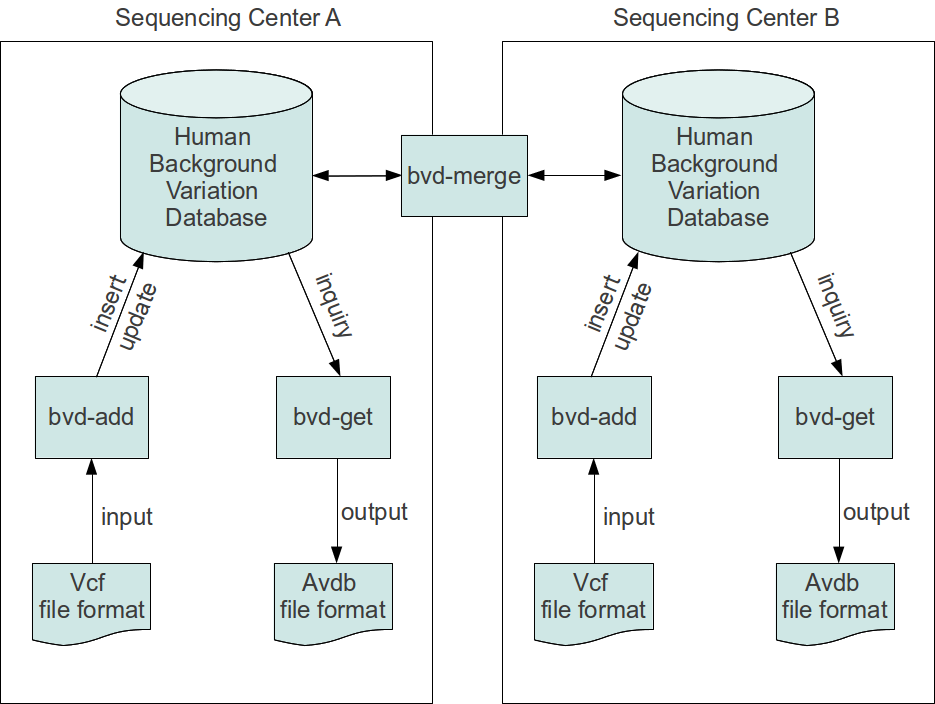
\includegraphics[scale=0.57]{fig_hbvdb_architecture.png}
\caption{Human Background Variantion Database architecture}
\label{fig:hbvdb_architecture}
\end{figure}



\section{Design and Coding Concept}
Because these tools are not aimed to be used by single person, but to be used by wide range of users, there are a couple of concepts that are embedded into the requirement of this project.
\begin{itemize}
\item \textbf{User friendly} - To allow all levels of users to use these tools. The only prior knowledge required is the purpose of these tools.
\item \textbf{Portable} - With the requirement to have more than one production site, these tools must not be specific to one machine. Installation must not require much effort. In the best case, the tools should be able to execute after download.
\item \textbf{Well-documented} - To allow the maintenance of these tools not to be restricted to one person.
\item \textbf{Robust} - It should be well-written enough to be handle exceptions.
\item \textbf{Command line interface} - These tools can be a part of any pipelines because of this feature.
\item \textbf{Product quality} - The package must have some procedures to make sure that these tools work correctly, according to specification.
\end{itemize} 



\section{Programming Language and Third Party Software}
With the requirement of these tools to be portable and command line interface, one of several suitable programming languages is Perl. Another reason to choose Perl is that the third party software used to parse the VCF files in this project is VCFtools. The advantage of using a Perl library in VCFtools, \emph{vcf.pm}, is how the VCF files are handled. With the VCFtools library, the one who maintain Human Background Variation Database project doesn't have to be concerned changes in the VCF format. As long as VCFtools is up-to-date, it will handle all these changes automatically.



\section{Main Functions}
\subsection{Bvd-add}
The purpose of \emph{bvd-add} is to transform variant information in VCF file into variant frequency and insert this into the database. One of the important features of this module is to allow users to add an \emph{exclude tag} to each variant in a dataset. This tag has a further use in \emph{bvd-get}. As the name imply, users can query variants frequency from the database by excluding certain tags. 

Another important feature here is that the users can specify their target database. Normally, variant frequencies parsed by this module will be sent to the default database. Having this feature will allow having more than one database in the same production site.

There are a few issues regarding writing operation found here. One is that users may accidentally execute \emph{bvd-add} for two times for one individual collection of variants. Another one is user errors, like executing \emph{bvd-add} with the wrong tags or the wrong VCF files. How can a user roll back the database if errors happen? And which of the database should users roll back to? The answer to all these issues can be found in Supported Features (section \ref{sec:support_features}).

\subsection{Bvd-get}
All variants frequencies in the database will be retrieved by default once \emph{bvd-get} is executed. By having features corresponding to \emph{bvd-add}, this module can retrieve variants frequencies that exclude some tags specified by users. Also, users can specify their source database if they don't want the frequencies from the default one.

\subsection{Bvd-merge} 
\emph{bvd-merge} is designed to combine the variants frequencies from another production site with the current site, the one that host this executable file. The input of this module is simply the location of the database of other production site. The issues here are the same with \emph{bvd-add} since it's also a writing operation. The solution can be found again in Supported Features (section \ref{sec:support_features}).



\section{Supported Features}
\label{sec:support_features}
The features here were not implemented separately, instead, they were embedded in the main modules. The reason that these features are separately described here is that they are implemented in more than one modules. Mainly, these features are related to writing operations which make changes to the database and may cause a lot of trouble if it isn't properly handled.

\subsection{Database Backup-Restore}
\label{sec:database_backup_restore}
Database backup and restore in this system is quite different from Database Management System (DBMS) which, normally, requires users to do the backup manually or automatically via some configuration. The concept here is very simple. Everytime, before the tools in this system perform writing operations, it will automatically perform a database backup first. The backup method is simply to make a copy of the database files with date-time suffix. The way to restore this backup file is to replace the current database files with the backup files that users want to restore.

The drawback of this feature is the usage of disk space because, by default, the backup is performed automatically in any writing operation. In this version of the tools, there is a parameter, \emph{--savediskspace}, to disable this automatically feature in each time these tools are executed. 

\subsection{Duplicated Individual-Variant File Checking}
\label{sec:duplicated_individual_variants_checking}
Users may accidentally try to insert variants from the same individual more than one time. To prevent this, these tools must detect if the content of the VCF file that is to be accessed is already in the system. The very straight forward way to prevent this is to keep the content of all inserted VCF files which can be used as an unique identifier for each VCF file inserted. Unfortunately, doing this may be against individuals' privacy. 

Our solution to this is to use a message digest, \emph{SHA512sum} which hashes the whole content of file and converts it into a string with certain length. Each of the inserted VCF files will be hashed and kept together with the database. Before a new VCF file is inserted into the database, its content will be hashed and evaluated to see if the hash value already exists in the system.

\subsection{Log File}
\label{sec:log_file}
The log file implemented in this system has a similar purpose to that of other systems. It keeps track of any crucial steps in any module. By having this feature, when users find out that something incorrect happened in the system, users can use this log file to trace back and roll back the database to the point where everything is correct.



\section{Testing Procedure}
Since the aim for these tools is to be widely used, we need to have something guarantee that every output is correct according to the specification. In the software development life cycle, testing is one of the mandatory steps that must be done to ensure the quality of the software. Two types of testing were performed in this project. One was unit test: the test to check if all the modules, \emph{bvd-add}, \emph{bvd-get} and \emph{bvd-merge}, work correctly according to specification. Another one was a performance test. This one checks if all the modules can be run in a real environment with a high workload. All the tests here were written in bash script so that they can be automatically executed using one single command. The list of test cases can be found in appendix \ref{sec:unit_test}.















\appendix
\addappheadtotoc
\chapter{Test Cases}
\label{chap:appendix_test_cases}

\section{Unit Test}
\label{sec:unit_test}
\definecolor{White}{rgb}{1,1,1}
\newcommand{\specialcell}[2][c]{%
  \begin{tabular}[#1]{@{}p{9.9cm}@{}}#2\end{tabular}}

\begin{longtable}{|c|l|l|}
\caption{Test cases of \emph{bvd-add}} 
\label{tab:test_cases_bvd_add} \\

\hline 
\multicolumn{1}{|c|}{\cellcolor{gray} \color{White} \textbf{Group}} & 
\multicolumn{1}{c|}{\cellcolor{gray} \color{White} \textbf{Case Name}} & 
\multicolumn{1}{c|}{\cellcolor{gray} \color{White} \textbf{Description}} \\ \hline 
\endfirsthead

\multicolumn{3}{c}%
{{\bfseries \tablename\ \thetable{} -- continued from previous page}} \\
\hline 
\multicolumn{1}{|c|}{\cellcolor{gray} \color{White} \textbf{Group}} & 
\multicolumn{1}{c|}{\cellcolor{gray} \color{White} \textbf{Case Name}} & 
\multicolumn{1}{c|}{\cellcolor{gray} \color{White} \textbf{Description}} \\ \hline 
\endhead

\hline \multicolumn{3}{|r|}{{Continued on next page}} \\ \hline
\endfoot

\hline \hline
\endlastfoot

\multirow{1}{*}{1} 
	& case\_bvd\_add\_08 & 
	\specialcell{1. To test bvd-add with real variants with random CHROM and POS from vcf file. \\
		2. To test if there isn't any existing bvdb database.\\
		3. To test if database '-d' is not presented\\
		4. To test if tags '-T' is not presented.} \\ \cline{2-3}
	& case\_bvd\_add\_01 & 
	\specialcell{1. To test bvd-add with real variants with random CHROM and POS from vcf file. \\
		2. To test if there isn't any existing bvdb database. \\
		3. To test if database '-d' is not presented. \\
		4. To test if tags '-T' is presented.} \\
\hline
\multirow{1}{*}{2} 
	& case\_bvd\_add\_02 & 
	\specialcell{Using data from case\_bvd\_add\_08 \\
		1. To test bvd-add with real variants with random CHROM and POS from vcf file. \\
		2. To test if it has existing bvdb database. \\
		3. To test if database '-d' is not presented. \\
		4. To test if no tags in current database. \\
		5. To test if tags '-T' is not presented.} \\ \cline{2-3}
	& case\_bvd\_add\_09 & 
	\specialcell{Using data from case\_bvd\_add\_08\\
		1. To test bvd-add with real variants with random CHROM and POS from vcf file. \\
		2. To test if it has existing bvdb database.\\
		3. To test if database '-d' is not presented.\\
		4. To test if no tags in current database.\\
		5. To test if tags '--tag' is presented.} \\ \cline{2-3}
	& case\_bvd\_add\_10 & 
	\specialcell{Using data from case\_bvd\_add\_01\\
		1. To test bvd-add with real variants with random CHROM and POS from vcf file. \\
		2. To test if it has existing bvdb database.\\
		3. To test if database '-d' is not presented.\\
		4. To test if there are tags in current database.\\
		5. To test if tags '-T' is not presented.} \\ \cline{2-3}
	& case\_bvd\_add\_11 & 
	\specialcell{Using data from case\_bvd\_add\_01\\
		1. To test bvd-add with real variants with random CHROM and POS from vcf file. \\
		2. To test if it has existing bvdb database.\\
		3. To test if database '-d' is not presented.\\
		4. To test if there are tags in current database.\\
		5. To test if tags '-T' is presented.} \\
\hline
\multirow{1}{*}{3} 
	& case\_bvd\_add\_03 & 
	\specialcell{To test the validity of frequency calculation as well as the order of the data for all possible case that can happen from individual variant files. \\
		There are 2 groups of data here\\
		1. Real data from 200danes database\\
		2. Synthetic data which is modified from some varaints in 200danes database} \\
\hline
\multirow{1}{*}{4} 
	& case\_bvd\_add\_04 & 
	\specialcell{To test with all possible combination of tags for each variant. There are 8 vcf files for all expected combination.} \\
\hline
\multirow{1}{*}{5} 
	& case\_bvd\_add\_05 & 
	\specialcell{To test with multi column vcf file. The input variants are the same with those from case\_bvd\_add\_03 but, instead of in separated vcf files, variants are combined into one single multicolumn vcf file.} \\
\hline
\multirow{1}{*}{6} 
	& case\_bvd\_add\_06 & 
	\specialcell{1. To test bvd-add with real variants with random CHROM and POS from vcf file. \\
		2. To test if there isn't any existing bvdb database.\\
		3. To test if database '-d' is presented.} \\
\hline
\multirow{1}{*}{7} 
	& case\_bvd\_add\_07 & 
	\specialcell{1. To test bvd-add with real variants with random CHROM and POS from vcf file. \\
		2. To test if it has existing bvdb database.\\
		3. To test if parameter '--database' is presented.} \\
\hline
\multirow{1}{*}{8} 
	& case\_bvd\_add\_12 & 
	\specialcell{To handle some strange characters in GT fields, '.'.} \\
\hline
\multirow{1}{*}{9} 
	& case\_bvd\_add\_13 & 
	\specialcell{Test if the database system, both database itself and message digest, are properly backup.} \\
\hline
\multirow{1}{*}{10} 
	& case\_bvd\_add\_14 & 
	\specialcell{Test if the parameter '-s' is presented.} \\ \cline{2-3}
	& case\_bvd\_add\_15 & 
	\specialcell{Test if the parameter '--savediskspace' is presented.} \\
\end{longtable}

\begin{longtable}{|c|l|l|}
\caption{Test cases of \emph{bvd-get}} 
\label{tab:test_cases_bvd_get} \\

\hline 
\multicolumn{1}{|c|}{\cellcolor{gray} \color{White} \textbf{Group}} & 
\multicolumn{1}{c|}{\cellcolor{gray} \color{White} \textbf{Case Name}} & 
\multicolumn{1}{c|}{\cellcolor{gray} \color{White} \textbf{Description}} \\ \hline 
\endfirsthead

\multicolumn{3}{c}%
{{\bfseries \tablename\ \thetable{} -- continued from previous page}} \\
\hline 
\multicolumn{1}{|c|}{\cellcolor{gray} \color{White} \textbf{Group}} & 
\multicolumn{1}{c|}{\cellcolor{gray} \color{White} \textbf{Case Name}} & 
\multicolumn{1}{c|}{\cellcolor{gray} \color{White} \textbf{Description}} \\ \hline 
\endhead

\hline \multicolumn{3}{|r|}{{Continued on next page}} \\ \hline
\endfoot

\hline \hline
\endlastfoot

\multirow{1}{*}{1} 
	& case\_bvd\_get\_02 & 
	\specialcell{To test with all possible combinations of normal excluded tags by using tags and variants generate from case\_bvd\_add\_04\\\\

		There are 3 tags in case\_bvd\_add\_04\\
		- colon\_cancer\\
		- lung\_cancer\\
		- prostate\_cancer\\\\

		So it has 16 possible normal combinations\\
		1. <no excluded tags>\\
		2. colon\_cancer\\
		3. colon\_cancer,lung\_cancer\\
		4. colon\_cancer,lung\_cancer,prostate\_cancer\\
		5. colon\_cancer,prostate\_cancer\\
		6. colon\_cancer,prostate\_cancer,lung\_cancer\\
		7. lung\_cancer\\
		8. lung\_cancer,colon\_cancer\\
		9. lung\_cancer,colon\_cancer,prostate\_cancer\\
		10. lung\_cancer,prostate\_cancer\\
		11. lung\_cancer,prostate\_cancer,colon\_cancer\\
		12. prostate\_cancer\\
		13. prostate\_cancer,colon\_cancer\\
		14. prostate\_cancer,colon\_cancer,lung\_cancer\\
		15. prostate\_cancer,lung\_cancer\\
		16. prostate\_cancer,lung\_cancer,colon\_cancer\\\\

		This testcase consist of 16 sub testcases. Each represent one combination above.\\\\

		Side note : Those 16 combinations can be reduced to 8 actual combinations\\
		a. <no excluded tags>\\
		b. colon\_cancer\\
		c. colon\_cancer,lung\_cancer\\
		d. colon\_cancer,lung\_cancer,prostate\_cancer\\
		e. colon\_cancer,prostate\_cancer\\
		f. lung\_cancer\\
		g. lung\_cancer,prostate\_cancer\\
		h. prostate\_cancer.} \\
\hline
\multirow{1}{*}{2} 
	& case\_bvd\_get\_01 & 
	\specialcell{To test with some variants in different chromosome from real data and also with some expected tags.} \\ \cline{2-3}
	& case\_bvd\_get\_05 & 
	\specialcell{Same as case\_bvd\_get\_01 but with parameter '-d' presented} \\ \cline{2-3}
	& case\_bvd\_get\_06 & 
	\specialcell{Same as case\_bvd\_get\_01 but with parameter '--database' presented} \\
\hline
\multirow{1}{*}{3} 
	& case\_bvd\_get\_03 & 
	\specialcell{This is the extension from case\_bvd\_get\_02. The purpose is to test with a weird excluded-tags combination.\\
		Only one case so far: lung\_cancer, colon\_cancer, lung\_cancer\\
		Data here are from case\_bvd\_add\_04} \\
\hline
\multirow{1}{*}{4} 
	& case\_bvd\_get\_04 & 
	\specialcell{This is the extension from case\_bvd\_get\_02. The purpose is to test with two tags, one tag that exist in database and another not exist.\\
		Only one case so far: lung\_cancer, breast\_cancer\\
		Data here are from case\_bvd\_add\_04} \\
\end{longtable}

\begin{longtable}{|c|l|l|}
\caption{Test cases of \emph{bvd-merge}} 
\label{tab:test_cases_bvd_merge} \\

\hline 
\multicolumn{1}{|c|}{\cellcolor{gray} \color{White} \textbf{Group}} & 
\multicolumn{1}{c|}{\cellcolor{gray} \color{White} \textbf{Case Name}} & 
\multicolumn{1}{c|}{\cellcolor{gray} \color{White} \textbf{Description}} \\ \hline 
\endfirsthead

\multicolumn{3}{c}%
{{\bfseries \tablename\ \thetable{} -- continued from previous page}} \\
\hline 
\multicolumn{1}{|c|}{\cellcolor{gray} \color{White} \textbf{Group}} & 
\multicolumn{1}{c|}{\cellcolor{gray} \color{White} \textbf{Case Name}} & 
\multicolumn{1}{c|}{\cellcolor{gray} \color{White} \textbf{Description}} \\ \hline 
\endhead

\hline \multicolumn{3}{|r|}{{Continued on next page}} \\ \hline
\endfoot

\hline \hline
\endlastfoot

\multirow{1}{*}{1} 
	& case\_bvd\_merge\_01 & 
	\specialcell{To test if one of the two given databases does not exist} \\
\hline
\multirow{1}{*}{2} 
	& case\_bvd\_merge\_02 & 
	\specialcell{To test if the one of the input databases doesn't have the database file} \\
\hline
\multirow{1}{*}{3} 
	& case\_bvd\_merge\_03 & 
	\specialcell{To test if the one of the input databases doesn't have the message-digest file} \\
\hline
\multirow{1}{*}{4} 
	& case\_bvd\_merge\_04 & 
	\specialcell{To test function 'validate\_bvdb' from command line with the database and without database file} \\
\hline
\multirow{1}{*}{5} 
	& case\_bvd\_merge\_05 & 
	\specialcell{To test if\\
		1. Local database exist with default location\\
		2. Some of the content from the input databases was already in the current local database} \\ \cline{2-3}
	& case\_bvd\_merge\_06 & 
	\specialcell{To test if\\
		1. Local database exist with default location\\
		2. Some of the content from the input databases was duplicated with each other} \\ \cline{2-3}
	& case\_bvd\_merge\_07 & 
	\specialcell{To test if\\
		1. Local database does not exist\\
		2. Some of the content from the input databases was duplicated with each other} \\ \cline{2-3}
	& case\_bvd\_merge\_09 & 
	\specialcell{To test if\\
		1. Local database exist with location from '-d' parameter\\
		2. Some of the content from the input databases was already in the current local database} \\
\hline
\multirow{1}{*}{6} 
	& case\_bvd\_merge\_08 & 
	\specialcell{To test with some variants in different chromosome from real data in. And also with some expected tags. With following conditions\\
		1. 2 vcf files in default local database.\\
		2. 2 vcf files in the first input database.\\
		3. 1 vcf file in the second input database.} \\ \cline{2-3}
	& case\_bvd\_merge\_10 & 
	\specialcell{To test with some variants in different chromosome from real data in. And also with some expected tags. With following conditions\\
		1. 2 vcf files in local database specified by parameter '-d'.\\
		2. 2 vcf files in the first input database.\\
		3. 1 vcf file in the second input database.} \\ \cline{2-3}
	& case\_bvd\_merge\_11 & 
	\specialcell{To test with some variants in different chromosome from real data in. And also with some expected tags. With following conditions\\
		1. No default local database.\\
		2. 3 vcf files in the first input database.\\
		3. 2 vcf file in the second input database.\\
		4. Output to default local database.} \\ \cline{2-3}
	& case\_bvd\_merge\_12 & 
	\specialcell{To test with some variants in different chromosome from real data in. And also with some expected tags. With following conditions\\
		1. No default local database.\\
		2. 3 vcf files in the first input database.\\
		3. 2 vcf file in the second input database.\\
		4. Output to local database specified by parameter '-d'.} \\
\hline
\multirow{1}{*}{7} 
	& case\_bvd\_merge\_13 & 
	\specialcell{To compare the result of bvd-add and bvd-merge with 5 real vcf files with expect tags. In bvd-merge, it'll merge the data from 5 databases, including the local one.} \\
\hline
\multirow{1}{*}{8} 
	& case\_bvd\_merge\_14 & 
	\specialcell{Test if the parameter '-s' is presented} \\ \cline{2-3}
	& case\_bvd\_merge\_15 & 
	\specialcell{Test if the parameter '--savediskspace' is presented} \\
\hline
\multirow{1}{*}{9} 
	& case\_bvd\_merge\_16 & 
	\specialcell{To test if the database is properly backup} \\
\end{longtable}

\section{Performance Test}
\label{sec:performance_test}

\begin{longtable}{|c|l|l|}
\caption{Test cases of performance test} 
\label{tab:test_cases_bvd_merge} \\

\hline 
\multicolumn{1}{|c|}{\cellcolor{gray} \color{White} \textbf{Group}} & 
\multicolumn{1}{c|}{\cellcolor{gray} \color{White} \textbf{Case Name}} & 
\multicolumn{1}{c|}{\cellcolor{gray} \color{White} \textbf{Description}} \\ \hline 
\endfirsthead

\multicolumn{3}{c}%
{{\bfseries \tablename\ \thetable{} -- continued from previous page}} \\
\hline 
\multicolumn{1}{|c|}{\cellcolor{gray} \color{White} \textbf{Group}} & 
\multicolumn{1}{c|}{\cellcolor{gray} \color{White} \textbf{Case Name}} & 
\multicolumn{1}{c|}{\cellcolor{gray} \color{White} \textbf{Description}} \\ \hline 
\endhead

\hline \multicolumn{3}{|r|}{{Continued on next page}} \\ \hline
\endfoot

\hline \hline
\endlastfoot

\multirow{1}{*}{bvd-add} 
	& case\_performance\_01 & 
	\specialcell{To see how well bvd-add be able to add variants from 200 real vcf files.} \\ \cline{2-3}
	& case\_performance\_02 & 
	\specialcell{To see if Bvd-add can handle large DB, 256,000,000 variants} \\ \cline{2-3}
	& case\_performance\_03 & 
	\specialcell{To see if Bvd-add can handel DB with expected number of tags,100,000 variants with 1,000 tags} \\ \hline
\multirow{1}{*}{bvd-get} 
	& case\_performance\_04 & 
	\specialcell{To see if Bvd-get can handel DB with expected number of tags, 100,000 variants with 1,000 tags, number of excluded tags = 100} \\ \cline{2-3}
	& case\_performance\_05 & 
	\specialcell{same as case\_performance\_04 but more extreme, number of excluded tags = 999 and not sorted} \\ 
\end{longtable}

\end{document}
